% !TEX TS-program = xelatex
% !TEX encoding = UTF-8 Unicode

\documentclass[11pt]{article}

\usepackage[top=20mm, bottom=20mm, left=20mm, right=20mm, a4paper]{geometry}
\usepackage{amsmath}
\usepackage{kotex}
\usepackage{listings}
\usepackage{setspace}
\usepackage{graphicx}
\usepackage{subcaption}
\usepackage{xcolor}
\usepackage[lighttt]{lmodern}
\usepackage{minted}
\usepackage{fontspec}


\usepackage{sourcecodepro}
\setmonofont[Scale=MatchLowercase]{JetBrains Mono}

\setmainhangulfont{NanumMyeongjo}
\setmainfont{Latin Modern Math}

\setmainfont{NanumMyeongjo}
\definecolor{GrayCodeBlock}{RGB}{241,241,241} 


\title{Wear OS를 이용한 심박수 측정 실험 보고서}
\author{20205178 박현}
\date{}

\renewcommand{\thesection}{\arabic{section}.\hspace{-10pt}}
\renewcommand{\thesubsection}{\arabic{section}. \arabic{subsection}.\hspace{-7pt}}
\usemintedstyle{manni}
\setminted{fontsize=\small, baselinestretch=1, bgcolor=GrayCodeBlock}
\definecolor{bg}{HTML}{282828}

% Document
\begin{document}
    \maketitle
    \setstretch{1.25}
    \section{실험 목적}
    본 실험은 시중에 쉽게 구할 수 있는 웨어러블 장치를 이용해 
    여러 명의 피실험자를 대상으로 심박수를 측정하여 이를 분석할 수 있는 
    환경을 구현해낼 수 있는가에 대한 것으로 크게 심박수를 측정하는 부분과
    측정된 데이터를 분석할 수 있도록 파일을 제공하는 부분으로 나뉜다. 
    
    \section{실험 방법}
    \subsection*{개발 과정}
    \hspace{0cm}
    \setstretch{0.0}
    \begin{description}
        \item[\hspace{0.5cm}기초적인 심박수 측정] SensorManager를 이용해 구현.
        \item[\hspace{0.5cm}권한 문제 해결] requestPermissions를 이용해 사용자 편의 향상.
        \item[\hspace{0.5cm}백그라운드 전환 시 중단 문제 해결] AmbientMode를 이용해 해결.
        \item[\hspace{0.5cm}파일 쓰기 문제 해결] 컨텍스트 객체의 filesDir 속성을 이용해 해결.
        \item[\hspace{0.5cm}외부에서 파일 접근 문제 해결] adb를 이용해 가져오는 것으로 해결.
        \item[\hspace{0.5cm}FTP 서버에 파일 전송] ftp4j 라이브러리를 이용해 구현.
    \end{description}
    \setstretch{1.25}
    \subsection*{실험 기구}
    \hspace{0cm}
    \setstretch{0.0}
    \begin{itemize}
        \item Samsung Galaxy A8 (SM-A530N) [ Android: 9 ]
        \item Samsung Galaxy Watch4 (SM-R860) [ System: 11, Wear OS: 3.5 ]
        \item TICKR FIT heart rate armband (WFBTHR03)
    \end{itemize}
    \setstretch{1.25}
    \subsection*{실험 절차}
    \hspace{0cm}
    \setstretch{0.0}
    \begin{enumerate}
        \item Galaxy Watch4에서 설정으로 들어가 디스플레이의 Always On Display를 활성화시킨다.
        \item 개발한 어플리케이션을 ADB를 이용해 Galaxy Watch4에 설치한다.
        \item Galaxy A8에서 위의 설치한 어플리케이션에 걸려 있는 백그라운드 제한을 해제한다.
        \item 기기들을 이용해 동시에 심박수를 측정한 후 FTP 서버에 측정된 결과 파일을 전송한다.
        \item FTP 서버에 저장된 파일을 읽어 파일 간 차이에 대해 분석해 유효성을 판단한다.
        \item[] \hspace{0.5cm}(이 때, 밴드의 경우 FTP 기능을 구현하지 않아 로깅에 사용된 휴대폰에서 파일을 가져온다.) 
    \end{enumerate}
    \setstretch{1.25}
    \newpage
    \section{실험 결과 및 과제}
    \subsection*{Standalone 상태 기기에서 심박수 측정의 불안정}
    \begin{figure}[!h]
        \centering
        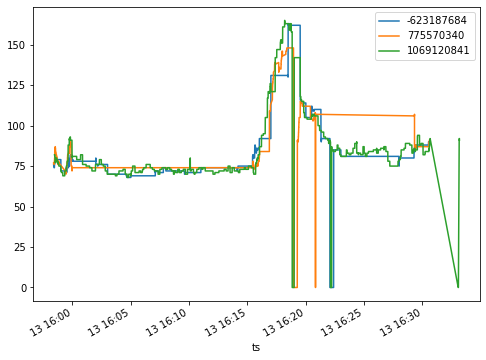
\includegraphics[width=8cm]{output.png}
        \caption{Galaxy Watch4를 이용한 심박수 측정 결과}
    \end{figure}
    \noindent
    775570340의 경우는 휴대폰과 연동이 안되어 Standalone 상태로 실험을 해
    다른 기기와는 달리 심박수 측정에 있어 정확한 측정이 되지 않은 것을 확인할 수 있었다.
    이에 이 문제점에 대한 가설로 백그라운드 제한을 해제하지 못했기 때문과
    Standalone 상태의 기기 좌측에 밴드를 여러 개 착용한 것이 원인으로 세웠다.
    이에 대한 실험을 후에 진행할 필요성이 있어 보인다.
    
    \subsection*{FTP 서버로의 파일 전송 시 에러 발생}
    모든 기기가 FTP 서버로 전송 시 튕기는 현상을 확인했으나 
    FTP 서버로의 전송만을 다시 실험한 결과 문제가 발생하지 않았다.
    이 문제점은 후에 단일 기기로 30분 동안 측정 후 FTP 서버로 데이터를 보낼 때
    Logcat을 통해 문제점을 재확인해야 할 필요성이 있어 보인다.
    \subsection*{Tickr-Logger에서의 타임스탬프 출력 문제}
    TICKR FIT의 경우 로깅 시 타임스탬프가 정상적으로 출력되지 않는 문제점을 발견하였다.
    이는 코드를 재분석한 결과 타임스탬프를 담당하는 변수가 0으로 초기화 후 
    재할당되지 않아 발생한 문제점으로 밝혀냈다. 이는 파일명에 첫 시작 시간이 기재되어 있고
    일정 시간 간격을 둬 로깅하기 때문에 실험에 있어 큰 문제는 없었을 것으로 예상되나
    편의 상 \texttt{System.currentTimeMillis()}를 활용해 문제를 해결할 것이다.
\end{document}
